\chapter{Analysis and Conclusions}
\label{analysis}

This chapter discusses the results. First, an evaluation is done on the workings
of wavelet analysis. Then the patterns found are evaluated. Next, the
survivability of projects with a certain patterns is evaluated. Then, the
answers on the research questions are presented. The last two sections describe
threats to validity and future work.

\section{Evaluation}
\subsection{Wavelet analysis}
\label{section:gapless_wavelets}
In verification of Hypothesis \ref{hyp:subsequent_data}, the requirement of a
subsequent data series for wavelet analysis, a hypothetical signal was
constructed. Let the following set of pairs be the signal $S$ to be analysed,
where the first entry is the time value, and the second entry the LOC value:
$$S = \{(1,100), (2,150), (5,250)\}$$

\noindent
In signal $S$ the two pairs having first entry $3$ and $4$ are missing. The
implementation of discrete wavelet transform in the 'wavelets' R package
requires an indexed series as input wavelet. This means, that whether or not
the signal contains gaps, these gaps are naturally closed by indexing the
signal. After zero-based indexing, the signal $S$ will look as follows:
$$S' = \{(0,100), (1,150), (2,250)\}$$

\noindent
The wavelet transformation can perfectly be done using $S'$ as input
signal. The output series of coefficients are indistinguishable from other
signals without gaps. However, the patterns found will be invalid as it ignored
intermediate data during similarity analysis.

\paragraph{}
A further investigation was done on how to fix such gaps. The use of four
different methods of 'guessing' the data was explored and the results were the
following:
\begin{description}
	\item[last observation carried] \hfill \\[1em]
	$S_{1} = \{(1,100), (2,150), (3,150), (4,150), (5,250)\}$

	\item[mean] \hfill \\[1em]
	$S_{2} = \{(1,100), (2,150), (3,200), (4,200), (5,250)\}$
	
	\item[piecewise constant interpolation] \hfill \\[1em]
	$S_{3} = \{(1,100), (2,150), (3,150), (4,250), (5,250)\}$
	
	\item[linear interpolation] \hfill \\[1em]
	$S_{4} = \{(1,100), (2,150), (3,183), (4,216), (5,250)\}$
\end{description}

\paragraph{}
The method \emph{last observation carried }\rm results in a signal with
same values between point 2 and 5, which shows a flat line when plotted in a
graph.

Filling the gaps with \emph{mean }\rm values, will also result in a signal with
same values. It is similar to last observation carried but using the mean is
excluding the two known observations, whereas last observation carried is
inclusive. Using mean, the number of second entries having same values
will therefore be smaller than using the last observation.

The \emph{piecewise constant }\rm interpolation results in a signal having two
smaller flat lines, because the repeating values are 'snapped' to the closest
neighbour.

Finally, the \emph{linear interpolation }\rm will result in a signal that
linearly flows towards the next known value. The advantage of this technique is
that there will not be a flat line in the signal, but the disadvantage is that
the numbers are new in the signal, possibly not even close to what was present
in the complete signal.

\paragraph{}
The flat lines introduced using the above techniques may be detected as no
change in LOC during that period. This is undesired as can be mistaken for a
pattern that stopped code evolution.

Moreover, the signal resulted from linear interpolation could be mistaken for
growth or decay in LOC, depending on the direction.

\paragraph{}
The success of one of the above methods of closing a gap depends on the size of
the gap. The smaller the gap, the lesser impact it has on the reliability of
the detection of a pattern for that particluar signal. The larger the gap, the
more the impact on reliability. Either way, adding data will add noise.
However, in general having gaps in the data and close the gaps by adding data
negatively influences the reliability of detecting patterns. Therefore,
Hypothesis \ref{hyp:subsequent_data} is confirmed.

\subsection{Patterns}
\label{section:pattern_evaluation}
There are more than 100,000 times more similar sequences found in the
scale/filter coefficients than in the wavelet/shift coefficients. The large
difference in number of sequences found between the two types of coefficients
is due to the fact that the LOC metric is a cumulative metric. The typical
trend of a LOC signal is growth. This makes finding similar sequences using
shift coefficients (i.e., along the time axis) less likely.

\paragraph{}
No patterns were detected in shift coefficients. This can be explained by the
fact that the 16 similar sequences in shift coefficients are not similar within
the same group of sequences.

Additionally, the shift coefficients are incomparable to the filter coefficients
because they were found in a fundamentally different way of signal
transformation. Mixing both types of coefficients would neglect the way the
coefficients were found and invalidate the patterns comprising sequences of
both types of coefficients.

\paragraph{}
The patterns that were detected show strong similarity. The similarity was
demonstrated in Figure \ref{figure:patterns_plots} in section
\ref{section:seqs_patterns}. The figure presented four graphs of four distinct
patterns plotted as wavelets of the original signals. Each graph contains
between 141 and 216 wavelets. Because of the similarity, the shape of the
pattern is still quite clear.

\subsection{Survivability}
\label{section:kp_survival}
The type A patterns would be the best candidates for being 'warning signs' as
they are detected at the end of evolution in dead projects. To determine whether
the chances for a project to die increase when having a type A pattern, two
groups are made. One group consisting of projects having the pattern, and
a second group of equal size consisting of projects not having the pattern.

Both groups of 93 projects contain alive and dead projects. The group with
projects without the pattern is representative to the data set as a whole.
Selecting projects and scoring for representativeness is done with the tool by
\citet{nagappan}. For each project of both groups it is recorded at what age
the project died, that is, if it died. For the others, the maximum age in the
data set is used. In Figure \ref{figure:kp_survival} the Kaplan-Meier
estimation of the survival function of the projects is shown for these groups.

\begin{figure}[H]
\caption{Kaplan-Meier estimation survival of projects regarding type A
patterns}\label{figure:kp_survival}
\centering
	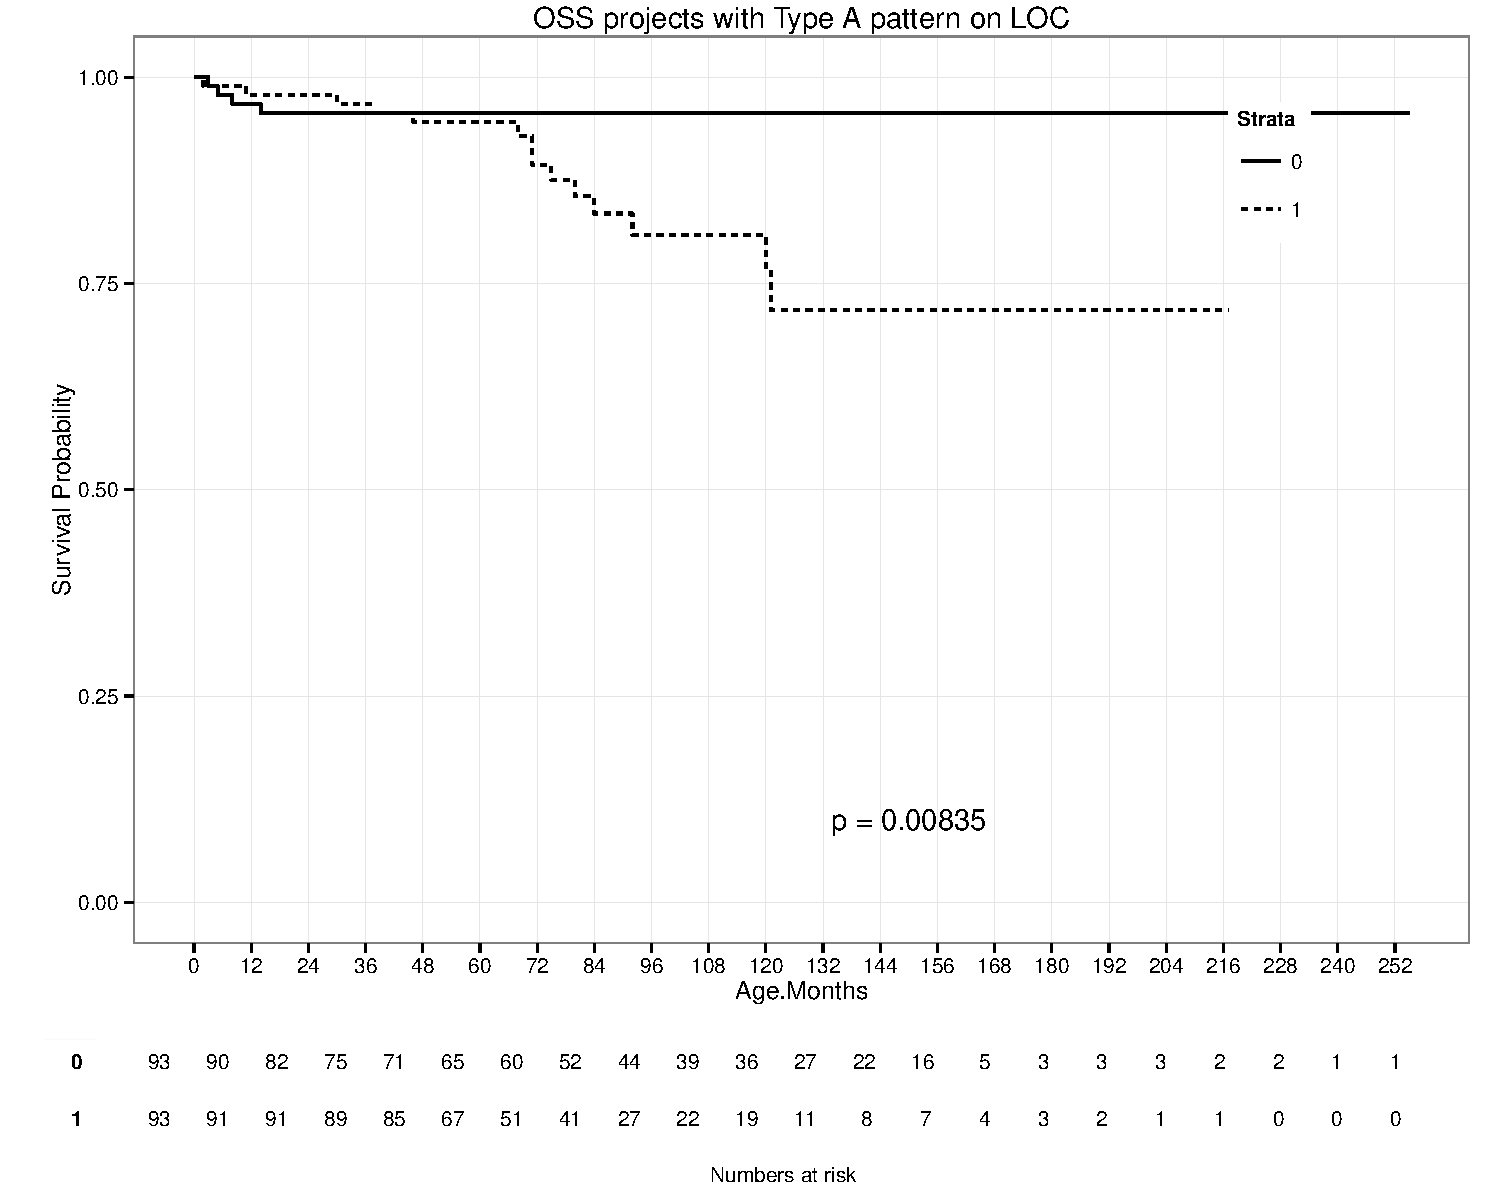
\includegraphics[width=386pt]{images/survival_LOC.pdf}
\end{figure}

\noindent
The Kaplan-Meier estimation of survival function of the projects as depicted in
Figure \ref{figure:kp_survival} suggests that projects in group 1 - the
projects having the type A pattern - die earlier than projects in group 0 - the
projects without the pattern. This suggests that having found a type A pattern
in a project shortens the project's life. Therefore, Hypothesis
\ref{hyp:pattern_types} is confirmed; projects with a pattern occurring at the
end of evolution of a dead project (i.e., type A pattern) have a higher chance
of dying.

\section{Conclusions}
\label{section:conclusions}
In this study, the patterns detected using wavelet analysis on LOC signals
comprise similar sequences of LOC series within and across projects. The
waveforms of these patterns vary in all kinds of shapes. The type A patterns
all show a stagnation of LOC changes, that is, very few changes relative to the
project size.

In general, the ability to detect a 'pattern' as being a group of similar
sequences within or across projects, depends on the similarity of the sequence
between other sequences within the same analysis. Therefore, it is important to
have a data set that is large enough and representative to the world of OSS
projects to be able to detect patterns that can be generalised
[\ref{itm:question_patterns}, \ref{itm:question_successfailure}].

\paragraph{}
Another aspect that contributes to the success or failure of wavelet analysis
for software evolution is that the input signal should be free of gaps. In
section \ref{section:gapless_wavelets} the confirmation of Hypothesis
\ref{hyp:subsequent_data} is argued.

In the case an input LOC signal for analysis is not continuous within the start
and end boundaries of the signal, the wavelet analysis will detect patterns
that are not trustworthy. Wavelet analysis may find more false-positive
evolutionary events [\ref{itm:question_successfailure}].

\paragraph{}
In this study, I have shown that wavelet analysis is able to find patterns that
increase the chances of a project to end. As discussed in section
\ref{section:kp_survival}, it appears that there is a relation between a
pattern of type A and the death of a project, however, it is not found to be a
causal relation.

Furthermore, as the patterns found during analysis are subject to the data set
as a whole, I cannot conclude that wavelet analysis is able to find
\emph{objective }\rm warning signs in OSS projects
[\ref{itm:question_warningsigns}].

\section{Threats to validity}
The following aspects were found which may lead to threats to the validity of
the results.

\begin{description}
	\item[Construct validity] \hfill
	
	\begin{description}
		\item[\rm{Missing historical data}] -- In the analysis of project's
			evolution data, only the data provided by the OhlohAnalytics tool was used.
			The data before the first data point in the set is not taken into account. It
			is possible that certain evolutionary events happened before the first point.
			These events were not detected as they lay beyond reach of this study.

		\item[\rm{Missing most recent data}] -- The data provided for the study has
			data points until June 2013. Therefore, not the most recent data of the
			projects is used.

		\item[\rm{LOC as activity indicator}] -- The use of LOC (defined as
			lines of code + comments + blanks) as a measure of project activity could be
			false. The LOC will not change between two months whenever the amount of code
			deleted is equal to the amount added. In that case, the churn would be twice
			the LOC added/deleted, but the LOC will stay the same.

			When patterns are detected that show a stagnation in LOC, the suggestion
			would be that the project's activity is decreasing. However, it might also
			be the case that by coincidence it seems activity is decreasing, but in
			reality lots of activity has been going on.

		\item[\rm{Data source}] -- Using only one data source (Ohloh) may
			influence the value of the metrics. Ohloh did the analysis of the project's
			source code repositories. Several studies have shown that the data provided
			by Ohloh needs a thorough examination and cleansing before it can be used
			\cite{bruntink2013, ohlohanalytics, bruntink2014}. The data was initially
			validated and cleansed, but to make it consistent. No actual verification on
			the correctness of the data was conducted.

	\begin{comment}
			Additionally, the data set of projects is a sample taken from all projects
			tracked by Ohloh. What is unclear is if the set of projects tracked by Ohloh
			is a representation of the world of OSS projects. Selecting a data set that
			is representative to the projects tracked by Ohloh does not automatically be
			representative to the world.

		\item[Sample size.] \hspace{1em} For this study, a set of 250 projects is
			used. Is this enough to generalise the results to the world of OSS projects.

		\item[Time resolution.] \hspace{1em} Is monthly aggregated data fine-grained
			enough?
	\end{comment}
	\end{description}

	\item[Internal validity] \hfill

	\begin{description}
		\item[\rm{Selection bias}] -- The selection criteria for the data was to have
			at least 12 data points. It turned out, no project in the set was younger
			than 14 months. It might be that these younger projects show significance in
			the ability to detect evolutionary events, possibly refute or confirm
			findings.
	\end{description}

	\item[External validity] \hfill

	\begin{description}
		\item[\rm{Replication}] -- It seems hard to precisely replicate the study
			as there are a multitude of possible configurations to be made that may, in
			the end, influence the results drastically. Such as, the definition of
			similarity between sequences (what deviation is allowed, what is the
			difference of coincidence and a reoccurring sequence), and the definition of
			a pattern (how many occurrences, minimum, and maximum length).
			
			Furthermore, there is the interpretation of what a 'warning sign' should
			look like on a pattern level.
	\end{description}
\end{description}

\section{Future work}
A next step in the research on the use of wavelet analysis for detecting
warning signs in software evolution would be to use a larger data set. It would
be interesting to know if the findings of the type A patterns will be
consistent. The whole usable data set for this study contains 5,986 projects
(section \ref{method:data}).

\paragraph{}
The analysis could be done on other signals. In this study, only LOC was used,
but many other signals can be constructed. LOC measures code activity to a
certain extent, but LOC churn could reflect code activity better. To use LOC
churn properly, the LOC modified fact is also needed.

Other metrics could be team size, developer's churn (the number of developers
added and removed from the team), contributor's code activity, bug reports,
defects per kLOC etc.

\begin{comment}
- Analyse results
- Conclude and interpret results
- Answer hypotheses and research questions
- Threats to validity
- Discussion
- Future work
 
This chapter contains the analysis and interpretation of the results. The
research questions are answered as best as possible given the results that were
obtained. The analysis also discussed parts of the questions that were left
unanswered.

An important topic is the validity of the results.
What methods of validation were used?
Could the results be generalized to other cases?
What threats to validity can be identified?

There is room here to discuss the results of related scientific literature here
as well.
How do the results obtained here relate to other work, and what consequences are
there?
Did your approach work better or worse?
Did you learn anything new compared to the already existing body of knowledge?
Finally, what could you say in hindsight on the research approach by followed?
What could have done better?
What lessons have been learned?
What could other researchers use from your experience?

A separate section should be devoted to ‘future work,’ i.e., possible extension
points of your work that you have identified. Other researchers (or yourself)
could use those as a starting point.

Refer to Chapters 3.7 and 4 in this example thesis at Paul’s
homepage\footnote{http://homepages.cwi.nl/~paulk/thesesMasterSoftwareEngineering/2006/ReneWiegers.pdf}.
\end{comment}
